\ifx\boi\undefined\ifx\problemname\undefined
\providecommand\sampleinputname{}
\providecommand\sampleoutputname{}
\documentclass[russian]{templates/boi}
\problemlanguage{.ru}
\fi
\newcommand{\boi}{Балтийская Олимпиада по Информатике}
\newcommand{\practicesession}{Тренировочный раунд}
\newcommand{\contestdates}{27 апреля - 1 мая, 2018}
\newcommand{\dayone}{День 1}
\newcommand{\daytwo}{День 2}
\newcommand{\licensingtext}{Задача публикуется под лицензией CC BY-SA 4.0.}
\newcommand{\problem}{Задача}
\newcommand{\inputsection}{Ввод}
\newcommand{\outputsection}{Вывод}
\newcommand{\interactivity}{Интерактивность}
\newcommand{\grading}{Оценивание}
\newcommand{\scoring}{Очки}
\newcommand{\constraints}{Ограничения}
\renewcommand{\sampleinputname}{Пример ввода}
\renewcommand{\sampleoutputname}{Пример вывода}
\newcommand{\sampleexplanation}[1]{Объяснение примера #1}
\newcommand{\sampleexplanations}{Объяснение примеров}
\newcommand{\timelimit}{Ограничение по времени}
\newcommand{\memorylimit}{Ограничение на память}
\newcommand{\seconds}{сек}
\newcommand{\megabytes}{MB}
\newcommand{\group}{Группа}
\newcommand{\points}{Очки}
\newcommand{\limitsname}{Ограничения}
\newcommand{\additionalconstraints}{Дополнительные ограничения}
\newcommand{\testgroups}{
Тесты разделены на группы. Очки за группу даются только если корректно решены все тесты в группе.
}
\fi
\def\version{jury-1}
\problemname{Двусторонний ток}
Фредерик играет с игрушечной железной дорогой, которую он сам сделал, чем очень гордится.
Дорога состоит из $N$ сегментов путей, соединённых по кругу, и пронумерованных $1, 2, \dots, N$ по часовой стрелке.
Электричество подается локомотиву через $M$ проводов, проложенных арками вдоль круга. Через каждый сегмент дороги проложен как минимум один провод.

Фредерику поднадоел наворачивающий круги поезд, и он решил добавить к каждому сегменту стрелочную развилку, чтобы устраивать поезду аварии, и прочим образом злобно развлекаться.
Стрелочные развилки, однако, нужно запитать электричеством, причем им подходит только специальный, \emph{двусторонний ток}.

По каждой арке проводов, проложенных вдоль путей, ток может течь в одном направлении -- либо по часовой, либо против часовой стрелки, причем Фредерик может выбрать подходящее направление.
Двусторонний ток можно получить, если подвести к сегменту ток и в одном, и в другом направлении (по двум разным проводам).

Таким образом, Фредерику нужно придумать, в какую сторону направить ток по каждому проводу, чтобы каждый сегмент путей был бы покрыт как минимум одним проводом с током, текущим по часовой стрелке, 
и одним проводом с током, текущим против часовой стрелки. Помоги Фредерику решить эту задачу.

\vspace{2mm}
%\hspace*{2mm}
\begin{center}
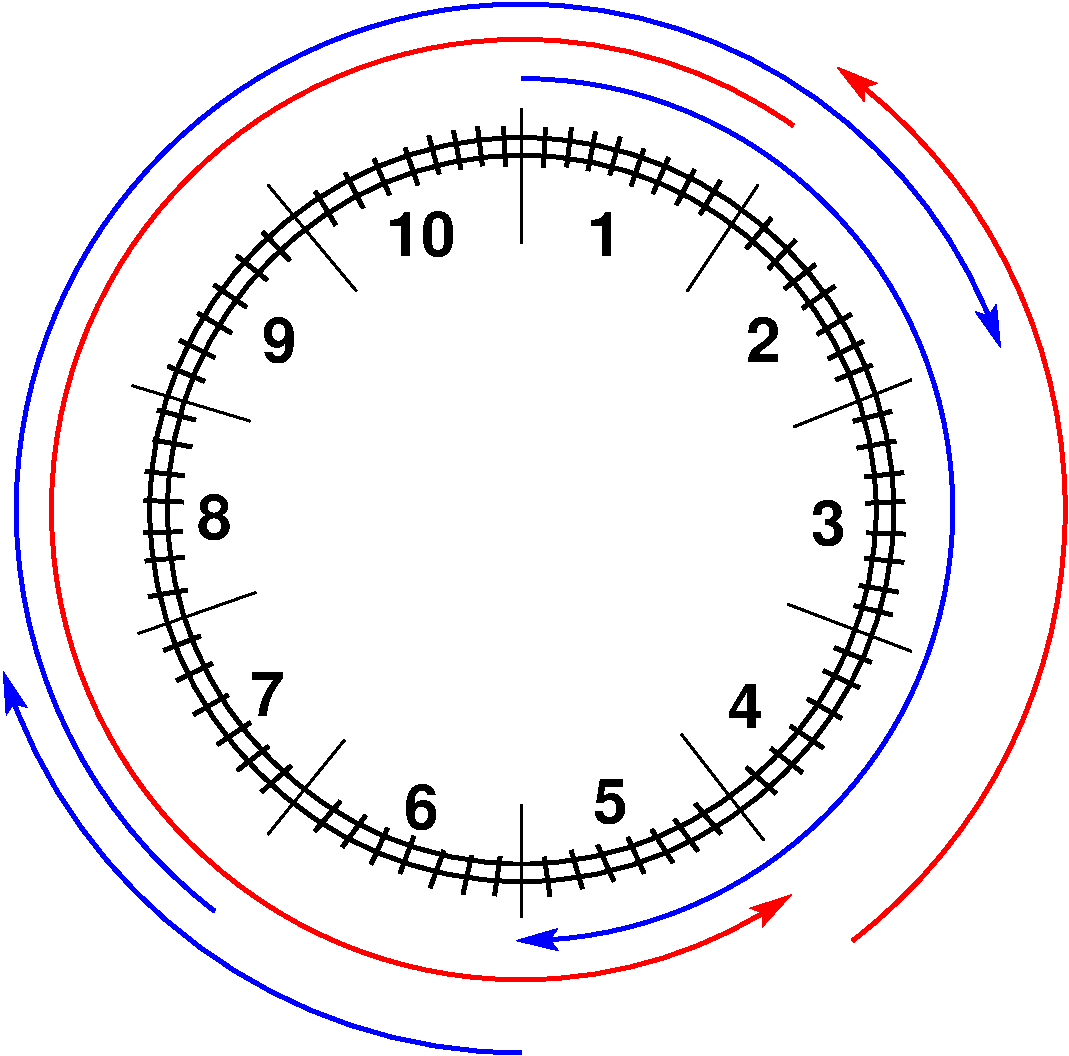
\includegraphics[width=0.5\textwidth]{alternatingfig.pdf}
\end{center}
\vspace{1mm}
{\em Решение первого примера. Стрелки вокруг железной дороги показывают провода, поставляющие электричество. Направление каждой стрелки соответствует выбранному Фредериком направлению тока (синий и красный цвет подчеркивают разные направления). Обратите внимание, что все стрелки можно развернуть, чтобы получить второе корректное решение: \texttt{11010}.}

\section*{\inputsection}
На первой строке даны два целых числа $N$ и $M$ -- количество сегментов железной дороги и количество проводов, соответственно.

На каждой из следующих $M$ строк даны два числа $1 \le a, b \le N$, указывающих, что имеется провод, покрывающий сегменты $a, a+1, \dots, b$.
Если $b$ меньше $a$, это значит что последовательность сегментов перескакивает через $N$, 
т.е. покрываются сегменты $a, \dots, N, 1, \dots, b$. Если $a=b$, то провод покрывает только один сегмент.

\section*{\outputsection}
На единственной строке вывести последовательность символов длиной $M$, состоящую из знаков \texttt{0} или \texttt{1}. $i$-тый символ должен быть равен \texttt{0}, если ток в $i$-том проводе нужно направить по часовой стрелке, и \texttt{1}, если ток нужно направить против часовой стрелки. Если существует несколько решений, вывести любое из них.

Если решений нет, вывести текст ``\texttt{impossible}''.

\section*{\constraints}
\testgroups

\noindent
\begin{tabular}{| l | l | l | l |}
\hline
\textbf{\group} & \textbf{\points} & \textbf{\limitsname} & \textbf{\additionalconstraints} \\ \hline
  1     & 13     & $2 \le N, M \le 15$ & \\ \hline
  2     & 20     & $2 \le N, M \le 100$ & \\ \hline
  3     & 22     & $2 \le N, M \le 1000$ & \\ \hline
  4     & 19     & $2 \le N, M \le 100\,000$ & Нет проводов с $b < a$. \\ \hline
  5     & 26     & $2 \le N, M \le 100\,000$ & \\ \hline
\end{tabular}

